\section{Analisis Kelayakan dan Proyeksi Dampak}
\label{sec:kelayakan}

\subsection{Asumsi Simulasi}

Simulasi memakai model tahunan PowerShift untuk 2026-2040. Baseline adalah phase down, yaitu PLTU IPP pensiun di akhir PPA, PLTU PLN pensiun di akhir umur desain, dan PLTS atap tumbuh mengikuti tren tanpa nilai ekspor. Asumsi utamanya adalah sebagai berikut. Seluruh parameter beserta sumber dan status verifikasinya tercantum pada Lampiran~\ref{lamp:asumsi}.
\begin{itemize}
  \item Produksi PLTS atap rata-rata 1.424 kWh/kWp/tahun, tertimbang penjualan listrik per provinsi \cite{D-GSA-PVOUT,D-PLN-STAT-2025}.
  \item Adopsi PLTS atap mengikuti kurva pangsa pasar terhadap waktu balik modal $\exp(-0{,}3 \times \text{payback})$ \cite{P-NREL-SOLARDS}, dibatasi kuota.
  \item Kompensasi pensiun dini PLTU IPP memakai estimasi skema ETM sebesar Rp1,045 miliar per MW per tahun percepatan, dikalibrasi ke refinancing Cirebon-1 US\$250-300 juta \cite{B-REUTERS-CIREBON-2022}. Untuk PLTU PLN, kompensasi berupa nilai buku yang hilang.
  \item Energi PLTU yang dipensiunkan digantikan PLTS atap tambahan dan sisa armada pada biaya marjinal batu bara DMO.
  \item Reserve margin dijaga 33\%. Kekurangan daya mampu dipenuhi pembangkit pengganti dengan biaya US\$120/kW/tahun.
  \item Nilai kesehatan US\$0,7 juta per kematian dini \cite{P-CREA-IESR-2023}.
\end{itemize}

\subsection{Penyaringan Kandidat Pensiun Dini}

Tabel~\ref{tab:kandidat} adalah keluaran tab Kandidat PLTU di PowerShift. Setiap PLTU dihitung seolah dipensiunkan sendiri pada 2031 dengan 80\% kompensasi dari dana luar.

\begin{table}[H]
\centering
\caption{Daftar urut kandidat pensiun dini 2031 menurut neraca negara per GW}
\label{tab:kandidat}
\resizebox{\textwidth}{!}{\begin{tabular}{rllrrrrrr}
\toprule
\# & PLTU & Pemilik & MW & Pensiun baseline & Neraca negara (Rp T) & Per GW (Rp T) & Dana luar (Rp T) & Kematian/tahun \\
\midrule
1 & Celukan Bawang & IPP & 426 & 2045 & 4,8 & 11,3 & 3,6 & 110 \\
2 & Paiton-3 & IPP & 815 & 2042 & 4,8 & 5,9 & 6,8 & 211 \\
3 & Cilacap Sumber & IPP & 2.260 & 2036 & 10,7 & 4,7 & 16,4 & 585 \\
4 & Tanjung Jati B & IPP & 4.640 & 2036 & 21,7 & 4,7 & 33,3 & 1.200 \\
5 & Cirebon & IPP & 1.584 & 2042 & 7,1 & 4,5 & 13,2 & 1.149 \\
6 & Serang & IPP & 660 & 2047 & 2,5 & 3,8 & 5,5 & 171 \\
7 & Jawa-7 & IPP & 1.982 & 2049 & 6,8 & 3,4 & 16,6 & 513 \\
8 & Batang (Central Java Power) & IPP & 1.900 & 2052 & 6,5 & 3,4 & 15,9 & 491 \\
9 & Paiton & PLN & 400 & 2033 & -0,8 & -2,0 & 0,7 & 103 \\
10 & Suralaya & PLN & 4.425 & 2036 & -14,9 & -3,4 & 25,9 & 1.144 \\
11 & Tanjung Awar-Awar & PLN & 700 & 2052 & -8,4 & -12,0 & 2,3 & 181 \\
12 & Pacitan & PLN & 630 & 2051 & -7,6 & -12,0 & 2,2 & 163 \\
13 & Rembang & PLN & 630 & 2051 & -7,6 & -12,0 & 2,2 & 163 \\
14 & Indramayu & PLN & 990 & 2050 & -11,9 & -12,0 & 3,5 & 256 \\
15 & Labuan & PLN & 600 & 2049 & -7,2 & -12,1 & 2,2 & 155 \\
16 & Pelabuhan Ratu & PLN & 1.050 & 2045 & -12,9 & -12,3 & 4,6 & 272 \\
17 & Lontar & PLN & 1.260 & 2051 & -16,1 & -12,8 & 4,0 & 326 \\
18 & Paiton Baru & PLN & 660 & 2052 & -9,4 & -14,2 & 2,2 & 171 \\
19 & Adipala & PLN & 660 & 2055 & -9,9 & -15,0 & 2,0 & 171 \\
\bottomrule
\end{tabular}
}
\sumber{PowerShift, tab Kandidat PLTU. Angka per PLTU mencakup seluruh unit yang belum pensiun di baseline pada 2032}
\end{table}

Pola yang muncul sangat jelas. Seluruh PLTU IPP memberi neraca negara positif karena PLN berhenti membayar kapasitas, sedangkan seluruh PLTU milik PLN memberi neraca negatif, umumnya Rp12-15 triliun per GW, karena biaya pengganti dan nilai buku tidak diimbangi penghematan pembayaran kapasitas. Karena itu, roadmap memilih PLTU IPP. Cirebon-1 dipilih sebagai percontohan Fase 2 karena beban kesehatannya tertinggi dan sudah memiliki kerangka ETM. Tanjung Jati B unit 1-2 dan Cilacap Phase I dipilih untuk Fase 3 karena berusia sekitar 25 tahun dan kontraknya mendekati akhir. Celukan Bawang memberi neraca per GW tertinggi dan melengkapi Fase 3.

\subsection{Hasil Roadmap}

Tabel~\ref{tab:hasil} dan Gambar~\ref{fig:neraca} menyajikan hasil tiga skenario roadmap dan dua komponen pembentuk roadmap lengkap.

\begin{table}[H]
\centering
\caption{Hasil kumulatif 2026-2040 terhadap baseline phase down}
\label{tab:hasil}
\resizebox{\textwidth}{!}{\begin{tabular}{lrrrrr}
\toprule
Indikator & Komponen PLTS atap & Komponen pensiun dini & Fase 1-2 & Roadmap Fase 1-3 & Varian seimbang \\
\midrule
Neraca PLN (Rp T) & -22,6 & 15,2 & -18,2 & -7,4 & 2,3 \\
Neraca negara, PLN + APBN (Rp T) & -27,1 & 15,2 & -22,8 & -11,9 & 1,8 \\
Dana luar ETM/JETP (Rp T) & 0,0 & 15,2 & 6,1 & 15,2 & 13,1 \\
Hemat tagihan pelanggan (Rp T) & 38,0 & 0,0 & 38,0 & 38,0 & 16,4 \\
CO$_2$ dihindari (Mt) & 30,5 & 4,9 & 28,9 & 35,4 & 15,2 \\
Kematian dini dihindari & 1.439 & 8.133 & 9.572 & 9.572 & 8.730 \\
Nilai kesehatan (Rp T) & 16,7 & 94,6 & 111,3 & 111,3 & 101,5 \\
PLTS atap 2040 (GWp) & 7,2 & 4,0 & 7,2 & 7,2 & 5,3 \\
Pembangkit pengganti (MW) & 0 & 3.006 & 660 & 3.006 & 2.580 \\
Kenaikan BPP maks. (Rp/kWh) & 7,7 & 0,0 & 6,8 & 5,6 & 2,4 \\
Pekerja PLTU terdampak & 0 & 1.366 & 300 & 1.366 & 1.173 \\
\bottomrule
\end{tabular}
}
\sumber{PowerShift, kartu angka dan tab Analisis}
\end{table}

\begin{figure}[H]
\centering
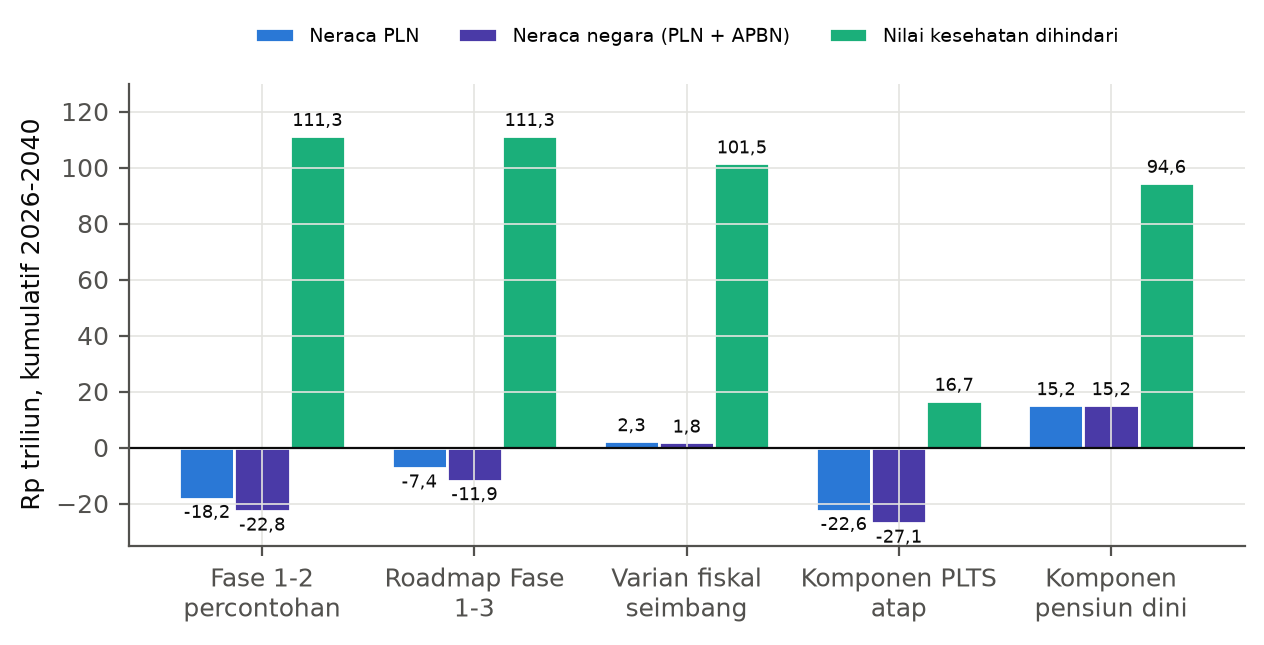
\includegraphics[width=\textwidth]{neraca_preset}
\caption{Neraca PLN, neraca negara, dan nilai kesehatan kumulatif 2026-2040}
\label{fig:neraca}
\sumber{PowerShift, tab Analisis bagian perbandingan skenario}
\end{figure}

Komponen PLTS atap saja membebani negara Rp27,1 triliun karena pendapatan PLN berpindah menjadi hemat tagihan pelanggan. Komponen pensiun dini saja memberi surplus Rp15,2 triliun. Roadmap lengkap menggabungkan keduanya sehingga beban negara turun menjadi Rp11,9 triliun, sementara manfaat kesehatan Rp111,3 triliun dan hemat tagihan pelanggan Rp38,0 triliun tetap diperoleh. Hasil skenario Fase 1-2 menunjukkan hal penting lain. Bila roadmap berhenti setelah percontohan, beban negara naik menjadi Rp22,8 triliun karena PLTS atap terus bertambah tanpa pensiun PLTU IPP berikutnya. Fase 3 karena itu bukan pilihan tambahan, melainkan bagian yang membuat program terjangkau.

\subsection{Biaya dan Skema Pembiayaan}

Tabel~\ref{tab:biaya} merinci arus biaya dan manfaat roadmap lengkap menurut pihak yang menanggung.

\begin{table}[H]
\centering
\caption{Arus biaya dan manfaat Roadmap Fase 1-3, kumulatif 2026-2040}
\label{tab:biaya}
\small
\begin{tabularx}{\textwidth}{L{3.2cm} Y r}
\toprule
Pihak & Pos & Rp triliun \\
\midrule
PLN & Pembayaran kapasitas PLTU IPP yang dihemat & +52,6 \\
 & Biaya energi yang dihemat & +17,9 \\
 & Pendapatan yang berpindah ke pemilik PLTS atap & -38,0 \\
 & Pembangkit pengganti 3.006 MW & -36,1 \\
 & Porsi PLN dari kompensasi (20\%) & -3,8 \\
 & \textbf{Neraca PLN} & \textbf{-7,4} \\
\addlinespace
APBN dan BUMN & Belanja PLTS atap gedung pemerintah dan BUMN & -33,8 \\
 & Tagihan listrik gedung yang dihemat & +32,8 \\
 & Insentif fiskal industri & -3,6 \\
\addlinespace
Negara & \textbf{PLN ditambah pos APBN} & \textbf{-11,9} \\
\addlinespace
Dana luar & Kompensasi pensiun dini (80\%) melalui ETM dan JETP & 15,2 \\
Pelanggan & Hemat tagihan pemilik PLTS atap & +38,0 \\
Masyarakat & Nilai kematian dini yang dihindari & +111,3 \\
\bottomrule
\end{tabularx}
\sumber{PowerShift, tab Neraca dan unduhan CSV}
\end{table}

Kewajiban PLTS atap gedung pemerintah dan BUMN hampir impas bagi APBN dalam horizon kajian dan berlanjut menguntungkan setelah 2040 karena tagihan terus dihemat. Beban negara bersih Rp11,9 triliun setara rata-rata kurang dari Rp1 triliun per tahun, kecil dibanding subsidi listrik sekitar Rp100 triliun per tahun \cite{B-KONTAN-SUBSIDI-2026}. Kebutuhan dana luar Rp15,2 triliun berada di bawah alokasi pensiun dini CIPP JETP yang sekitar US\$1,3 miliar atau Rp21,5 triliun \cite{P-CREA-CIPP-2023}.

\subsection{Proyeksi Dampak dan Capaian Indikator}

Tabel~\ref{tab:kpi} membandingkan hasil model dengan indikator keberhasilan laporan kelompok.

\begin{table}[H]
\centering
\caption{Capaian indikator keberhasilan per skenario}
\label{tab:kpi}
\small
\begin{tabular}{lrrr}
\toprule
Indikator & Fase 1-2 & Roadmap Fase 1-3 & Varian seimbang \\
\midrule
PLTU pensiun dini (GW) & 0,66 & 3,01 & 2,58 \\
Tambahan PLTS atap 2040 (GWp) & 3,19 & 3,19 & 1,30 \\
Rasio PLTS atap terhadap PLTU & 483\% & 106\% & 50\% \\
PLTS atap Jawa-Bali 2028 (MWp) & 1.363 & 1.363 & 1.250 \\
Kuota Jawa-Madura-Bali 2028 (MWp) & 1.850 & 1.850 & 1.850 \\
Dana luar (Rp T) & 6,1 & 15,2 & 13,1 \\
Alokasi pensiun dini CIPP JETP (Rp T) & 21,5 & 21,5 & 21,5 \\
Neraca negara (Rp T) & -22,8 & -11,9 & 1,8 \\
\bottomrule
\end{tabular}

\sumber{PowerShift, tab Indikator roadmap, target dari laporan kelompok \cite{L-LAPORAN-K17}, kuota dari \cite{B-CNBC-ROOFTOP-2028}, dan CIPP JETP \cite{P-CREA-CIPP-2023}}
\end{table}

Roadmap lengkap mencapai indikator kesetaraan. Tambahan PLTS atap 3,19 GWp melampaui 3,01 GW PLTU yang dipensiunkan. Pensiun dini 3,01 GW di Jawa-Bali juga melampaui target JETP nasional 1,7 GW. Kuota PLTS atap 2028 baru tercapai 74\% (1.363 dari 1.850 MWp) karena kewajiban baru berlaku pada 2028. Kuota ini dapat dikejar bila kewajiban gedung pemerintah dan BUMN dimulai pada akhir Fase 1.

Kesetaraan daya tidak sama dengan kesetaraan energi. Faktor kapasitas PLTS atap sekitar 16\%, sedangkan PLTU sekitar 64\%. Gambar~\ref{fig:substitusi} menunjukkan lintasannya per tahun. Selama 2031-2035, tambahan PLTS atap masih tertinggal dari kapasitas PLTU yang sudah pensiun, dengan selisih terbesar sekitar 1,1 GW pada 2035. Mulai 2036, Tanjung Jati B 1-2 dan Cilacap Phase I juga pensiun di baseline sehingga selisih terhadap baseline mengecil, sementara kewajiban dan insentif terus menambah PLTS atap. Tambahan PLTS atap melampaui kapasitas yang pensiun lebih awal sejak 2036 dan mencapai 106\% dari seluruh PLTU yang dipensiunkan pada 2040. Selisih selama Fase 3 ditutup pembangkit pengganti. Dari sisi energi, PLTS atap tambahan mengganti sekitar 31\% energi PLTU yang dipensiunkan. Sisanya dipasok pembangkit pengganti dan armada yang ada. Karena itu, indikator kesetaraan daya sebaiknya dilaporkan bersama indikator energi.

\begin{figure}[H]
\centering
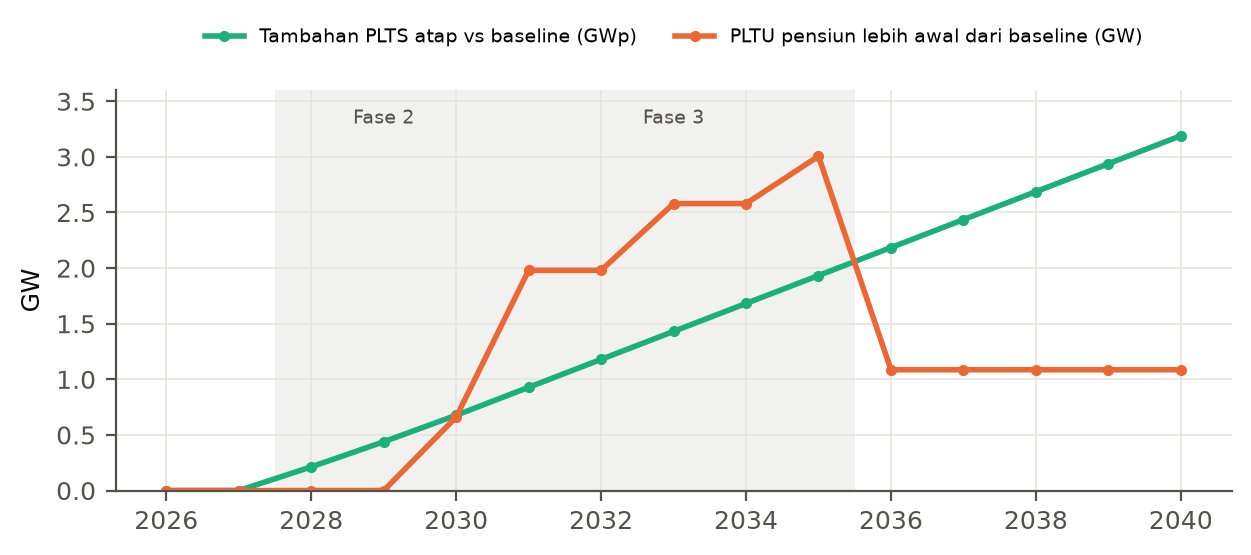
\includegraphics[width=\textwidth]{substitusi_roadmap}
\caption{Tambahan PLTS atap dan kapasitas PLTU pensiun dini per tahun pada Roadmap Fase 1-3}
\label{fig:substitusi}
\sumber{PowerShift, tab Indikator roadmap}
\end{figure}

\subsection{Keandalan Sistem}

\begin{figure}[H]
\centering
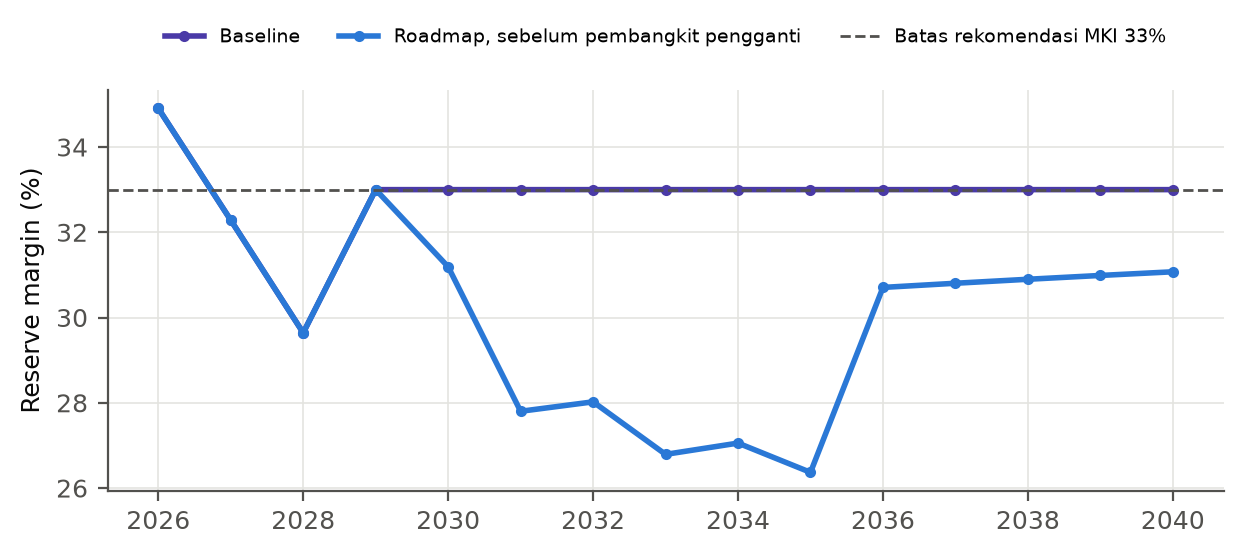
\includegraphics[width=\textwidth]{reserve_margin}
\caption{Reserve margin baseline dan Roadmap Fase 1-3 sebelum pembangkit pengganti}
\label{fig:rm}
\sumber{PowerShift, tab Keandalan, berdasarkan \cite{B-MATAHARI-2024,B-PETROMINDO-RESERVE}}
\end{figure}

Tanpa pembangkit pengganti, reserve margin roadmap turun dari 33\% menjadi 26,4\% pada 2035 (Gambar~\ref{fig:rm}). Kebutuhan pengganti mencapai 3.006 MW pada 2035 dan turun menjadi 1.086 MW setelah 2036 karena sebagian PLTU memang pensiun di baseline. Biaya pengganti sudah dihitung dalam neraca PLN. Rencana tambahan pembangkit Jamali dalam RUPTL 2025-2034 \cite{B-LISTRIKID-RUPTL-JAMALI} dapat dijadwalkan untuk mengisi kebutuhan ini.

\subsection{Sensitivitas}

\begin{figure}[H]
\centering
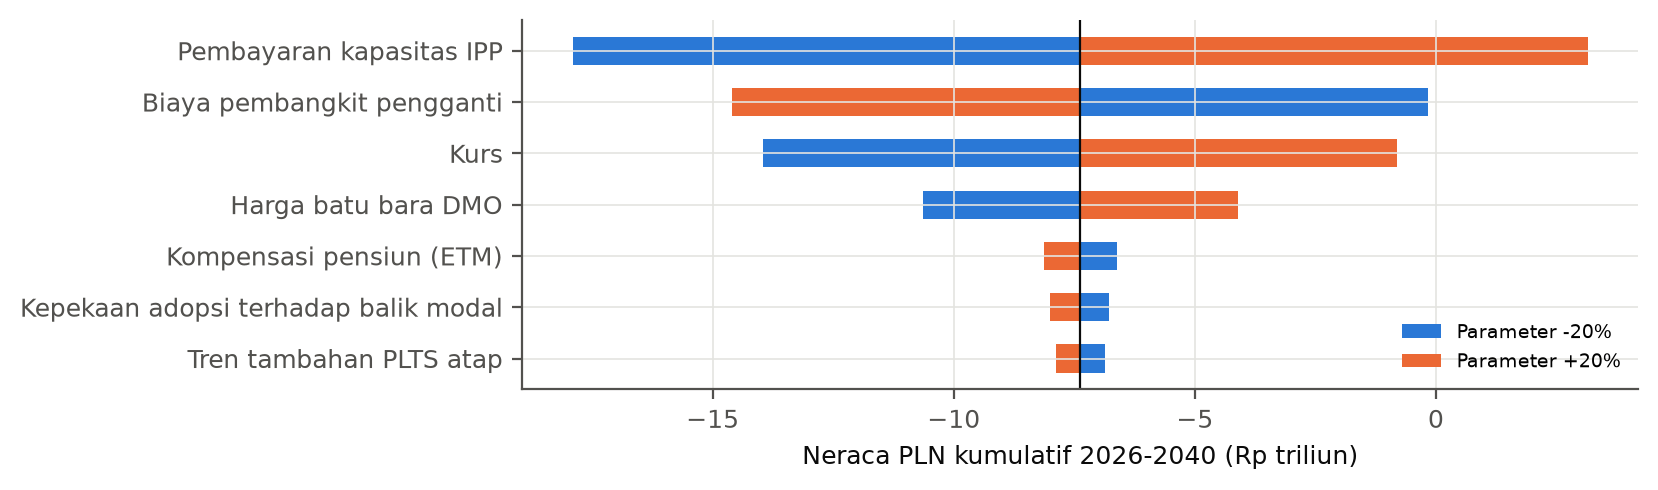
\includegraphics[width=\textwidth]{tornado_roadmap}
\caption{Sensitivitas neraca PLN Roadmap Fase 1-3 terhadap perubahan parameter $\pm$20\%}
\label{fig:tornado}
\sumber{PowerShift, tab Analisis bagian sensitivitas}
\end{figure}

Neraca PLN paling peka terhadap pembayaran kapasitas IPP, biaya pembangkit pengganti, dan kurs (Gambar~\ref{fig:tornado}). Bila pembayaran kapasitas 20\% lebih tinggi dari asumsi, neraca PLN berbalik positif Rp3,1 triliun. Kontrak IPP yang sebenarnya karena itu perlu dimasukkan PLN ke PowerShift sebelum keputusan.

Besaran kompensasi adalah risiko terbesar. Kajian ini memakai estimasi ETM yang dikalibrasi ke refinancing Cirebon-1. Bila kompensasi memakai valuasi ETP yang dirangkum laporan kelompok, beban negara menjadi Rp14,7 triliun dan kebutuhan dana luar Rp26,5 triliun, melampaui alokasi CIPP JETP. Bila memakai klaim PLN untuk Cirebon-1 (Rp60 triliun untuk lima tahun), beban negara menjadi Rp74,3 triliun. Tanpa dana luar sama sekali, beban negara Rp27,1 triliun. Angka-angka ini menegaskan bahwa syarat penutupan K4, yaitu kompensasi yang disepakati dan dana luar yang terikat lebih dulu, menentukan kelayakan program.

\subsection{Risiko dan Mitigasi}

\begin{table}[H]
\centering
\caption{Risiko pelaksanaan dan penanganannya}
\label{tab:risiko}
\small
\begin{tabularx}{\textwidth}{L{3cm} Y Y L{2.4cm}}
\toprule
Risiko & Dampak & Mitigasi & Penanggung jawab \\
\midrule
Klaim kompensasi jauh di atas estimasi & Beban negara dan dana luar membengkak, pensiun dibatalkan & Negosiasi berbasis nilai keuntungan yang hilang, syarat dana terikat sebelum penutupan (K4) & Kemenkeu, PLN \\
\addlinespace
Pembangkit pengganti terlambat & Reserve margin di bawah 33\% & Penutupan ditunda sampai pengganti beroperasi, pengganti masuk RUPTL & PLN, KESDM \\
\addlinespace
Adopsi PLTS atap di bawah target & Indikator kesetaraan tidak tercapai & Kewajiban gedung pemerintah dan BUMN sebagai lantai, insentif industri dinaikkan bila tertinggal & KESDM, Kemenkeu \\
\addlinespace
Integrasi PLTS atap mengganggu jaringan & Tegangan dan frekuensi tidak stabil di siang hari & Penguatan jaringan distribusi dan penyimpanan energi pada Fase 3 & PLN \\
\addlinespace
Pekerja tidak terserap & Penolakan lokal dan ketimpangan baru & Pelatihan ulang dimulai satu tahun sebelum penutupan (K5) & Kemenaker, Pemda \\
\addlinespace
Data kontrak IPP tidak terbuka & Hasil penyaringan meleset & PLN memasukkan data kontrak ke PowerShift secara tertutup, hasil agregat dibuka & PLN, Satgas \\
\bottomrule
\end{tabularx}
\end{table}
